\documentclass[12pt]{scrartcl}
\usepackage[english]{babel}
\usepackage[utf8x]{inputenc}
\usepackage{amsmath}
\usepackage{graphicx}
\usepackage[colorinlistoftodos]{todonotes}
% -MINE
\usepackage[a4paper, total={6in, 8in}]{geometry}
\usepackage{placeins}
\usepackage{subcaption}
\usepackage{enumerate}
\usepackage{gensymb}
\usepackage{hyperref}
\usepackage{pdfpages}
\usepackage{siunitx}
\usepackage{tikz}


\begin{document}

\begin{titlepage}

\newcommand{\HRule}{\rule{\linewidth}{0.5mm}} % Defines a new command for the horizontal lines, change thickness here

\center % Center everything on the page
 
%----------------------------------------------------------------------------------------
%	HEADING SECTIONS
%----------------------------------------------------------------------------------------

\textsc{\LARGE Politecnico di Milano}\\[1.5cm] % Name of your university/college
\textsc{\Large MSc in Mechanical Engineering}\\[0.5cm] % Major heading such as course name
\textsc{\large Functional Mechanical Design}\\[0.5cm] % Minor heading such as course title

%----------------------------------------------------------------------------------------
%	TITLE SECTION
%----------------------------------------------------------------------------------------

\HRule \\[0.4cm]
{ \huge \bfseries Turning pad subsystem}\\[0.4cm] % Title of your document
\HRule \\[1.5cm]
 
%----------------------------------------------------------------------------------------
%	AUTHOR SECTION
%----------------------------------------------------------------------------------------

% \begin{minipage}{0.4\textwidth}
% \begin{flushleft} \large
% Jai \textsc{Ummat}\\
% \end{flushleft}
% \end{minipage}
% ~
% \begin{minipage}{0.4\textwidth}
% \begin{flushright} \large
% Túlio Vinícius \textsc{Berbert Patriota}% Your name
% \end{flushright}
% \end{minipage}
Tulio Vinicius \textsc{Berbert Patriota} - 899666\\
Marco \textsc{Lorello} - \\
Samir \textsc{Hajili} - 
\\[2cm]

% If you don't want a supervisor, uncomment the two lines below and remove the section above
%\Large \emph{Author:}\\
%John \textsc{Smith}\\[3cm] % Your name

%----------------------------------------------------------------------------------------
%	DATE SECTION
%----------------------------------------------------------------------------------------

{\large \today}\\[1cm] % Date, change the \today to a set date if you want to be precise

%----------------------------------------------------------------------------------------
%	LOGO SECTION
%----------------------------------------------------------------------------------------
\centering

\includegraphics[width=6cm]{Pictures/logo.png}\\[1cm] % Include a department/university logo - this will require the graphicx package
 
%----------------------------------------------------------------------------------------

\vfill % Fill the rest of the page with whitespace

\end{titlepage}

\tableofcontents
\listoffigures
\listoftables
\newpage
\linespread{1.3}

\section{Introduction}
The subsystem has the purpose of discharging the soap once the product has been definitively made. The tilting pad motion is a pure rotation and takes place around a fixed axis. The movement is realized through a slider crank mechanism in which the slider is moved by a translating cam.
The slider has a mass of 2.3 \si{\kilo\gram} and the tilting pad is characterized by a momentum of inertia (with respect to the axis of rotation) $J =1.1 \si{\kilo\gram\metre\squared}$.
The motion law of the tilting pad is:
\begin{figure}[htbp!]
	\centering
	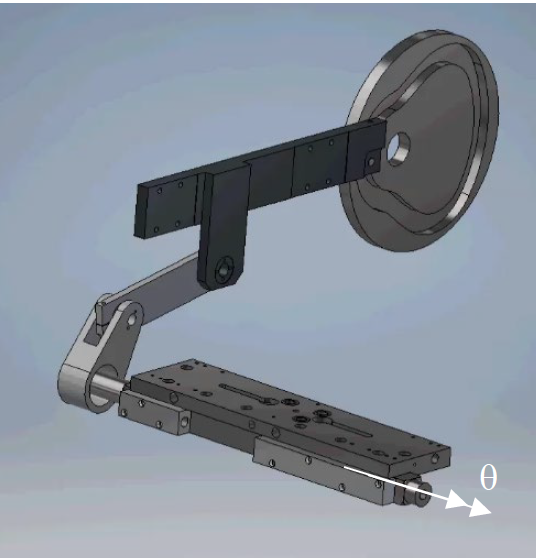
\includegraphics[width=0.6\textwidth]{Pictures/initial}
	\caption{Example of uploading subsystem.}
	\label{fig: initial system}
\end{figure}

The motion of the system has to achieve the points described by Tab.~\ref{tab: motion law}.
\begin{table}[htbp]
\centering
\begin{tabular}{|l|l|}
\hline
$\alpha = 0^\circ$  & $\theta = 45^\circ$ \\ \hline
$\alpha = 70^\circ$ &  $\theta = 0^\circ$ \\ \hline
  $\alpha = 200^\circ$  & $\theta = 0^\circ$  \\\hline
   $\alpha = 360^\circ$   &  $\theta = 45^\circ$ \\\hline
 \end{tabular}
\caption{Motion law}
\label{tab: motion law}
\end{table}

\section{Objectives}
Considering the driver unit moves at constant speed, we need to 
\begin{enumerate}[i]
	\item Design the motion law of the tilting pad.
	\item Synthesize the slider crank mechanism and the cam mechanisms with a translating follower.
	\item Analyse the mechanism through kinematic parameters (transmission angle, pressure angle and undercut) and compute the motion law obtained with the designed mechanism
	\item Calculate forces transmitted and the motor torque with a multibody model.
	\item Critically evaluate the feasibility of the system.
\end{enumerate}

\section{Methods and procedure}
The motion law is described for $\theta$. Since we are constructing a translating cam whose displacement $x$ is the displacement of the slider on the slider-crank mechanism. We first choose $a$, $b$, $e$ and $\alpha_0$, accounting for performance parameters as transmission angle $\mu$. From that, we obtain the desired motion law in $x$ and generate the corresponding cam.  
\subsection{Slider-crank}
\begin{figure}[htbp!]
\centering
	\begin{tikzpicture}[scale = 0.05]
		\draw[thick] (0,0) -- (-45.89,65.53);
		\filldraw[black] (0,0) circle(1);
		\draw[thick] (-45.89,65.53) -- (51.07,90);
		\filldraw[black] (-45.89,65.53) circle(1);
		\filldraw[black] (51.07,90) circle(1);
		\draw[dashed] (-45.89,65.53) -- (51.07,65.53);
		\draw[dashed] (-60,0) -- (60,0);
		\draw[dashed,thick] (-60,90) -- (60,90);
		\draw[->,thick] (10,0) arc(0:125:10);%(10,0) -- (-5.74,8.19);
		\node [above] at (10,9) {$\phi$};
		\draw[->,thick] (0,65.53) arc(0:14.1635:45.89);
		\node [above] at (5,65.53) {$\beta$};
		\node [left] at (-22,32) {$a$};
		\node [above] at (0,78) {$b$};
		\draw [|-|] (70,90) -- (70,0);
		\node [right] at (70,45) {$e$};
		\draw [|->,thick] (51.07,95) -- (65,95);
		\node [above] at (60,95) {$x$};
	\end{tikzpicture}
	\caption{Schematic of the slider-crank mechanism.} 
	\label{fig: slider crank}
\end{figure}
 With the motion described for $\theta$, we derive the motion for $x$ as (see Fig.~\ref{fig: slider crank})
\begin{eqnarray}
	x = a\sin(\phi) + b\cos(\beta),
\end{eqnarray}
where $a$ is the crank length, $b$ is the slider length, $e$ is the height of the slider with respect to the ground and
\begin{eqnarray}
\beta &=& \arcsin\left(\frac{e-a\sin(\phi)}{b}\right),\\
	&&\dots \phi = \phi_0 + \theta.
\end{eqnarray}
 We initially choose all the motions to be cycloidal, so the normalized motion law is
\begin{eqnarray}
	\left\{\begin{array}{l}
		\ddot{y} = c_a \frac{h}{t_a^2} \sin\left(\frac{2\pi t}{t_a} \right),\\
		\dot{y} = \frac{h}{t_a} \left[1 - \cos\left(\frac{2\pi t}{t_a}\right)\right],\\
		y = h \left[\frac{t}{t_a}-\frac{1}{2\pi}\sin\left(\frac{2\pi t}{t_a}\right) \right],
	\end{array} \right.
\end{eqnarray}
where $c_a = 2\,\pi$, $h$ is the lift from time $0$ until $t_a$. We can also describe the motion law with respect to the master angle ($\alpha$) and thus the $\dot{y} = y' \omega$ and $\ddot{y} = y'' \omega^2$, where $y'$ and $y''$ are the geometrical velocities and accelerations, respectively, and $\omega$ is the constant angular speed. The advantage of the cycloidal motion is that because the relationship between $x$ and $\theta$ are trigonometric, both the motions will be cycloidal (not true if I choose a different motion for $\theta$, let's say, cubic).

The crank $a$ length should be long enough so that low forces are needed to rotate the inertia but short enough to avoid oversizing. For a giving $a$, the eccentricity $e$ should be close to $a$ to ensure a high transmission ratio. For the case we chose $e>a$; in this way we won't meet a dead center during the working condition. The coupler length $b$ is chosen larger so that a significant displacement $x$ takes place for the given angular displacement.

\subsection{Cam design}
For the design of the first cam, we use the obtained motion law for $X$ and consider the equations for a translating cam with a roller. First, we find the pressure angle $\phi$ as
\begin{eqnarray}
	\phi = \frac{X'}{R_{b0} + X},
\end{eqnarray}
where $X' = \partial X /\partial \alpha$ is our geometrical velocity (remember the abscissa is the master angle $\alpha$) and $R_{b0}$ is the base radius of the cam. The next step is to find the pitch profile. The curvature radius of the pitch profile is found by 
\begin{eqnarray}
	\rho_0 = \frac{\left[X'^2+ (R_{b0} + X)^2\right]^{3/2}}{(R_{b0} + X)^2 - (R_{b0} + X)X'' + 2X'^2},
\end{eqnarray}
while the curvature radius of the cam profile is 
\begin{eqnarray}
	\rho = \rho_0 - Rr,
\end{eqnarray}
where $R_r$ is the roller radius.

 Using Carnot theorem, one can find the polar coordinates of the cam as
\begin{eqnarray}
	r(\alpha) &=& \sqrt{R_r^2+ (R_{b0}+ X)^2- 2Rr(R_{b0} + X)\cos \phi},\\
	\varphi(\alpha) &=& \alpha + \arcsin \left(\frac{R_r \sin \phi}{r}\right).
	\label{exp: cam profile}
\end{eqnarray}

After the definition of the cam and of the slider-crank mechanism, their profile was designed through MATLAB routines. The physical object of the cam, that will later be used in ADAMS, was constructed into a CAD software, SolidWorks, from the profiles given by the MATLAB routine.

\section{ADAMS analysis}

\section{Results}

We choose the following parameters for the slider-crank mechanism
\begin{eqnarray*}
	a &=& \SI{80}{\milli\metre}, \qquad b = \SI{100}{\milli\meter}, \qquad e = \SI{90}{\milli\metre}, \qquad \phi_0 = 125^\circ.	
\end{eqnarray*}


The resulting motion law is depicted at Fig.~\ref{fig: cic motion laws}. We chose the cycloidal motion law for it has no discontinuities at high derivatives (until acceleration), favoring the smoothness of the system.
\begin{figure}[htbp!]
	\centering
	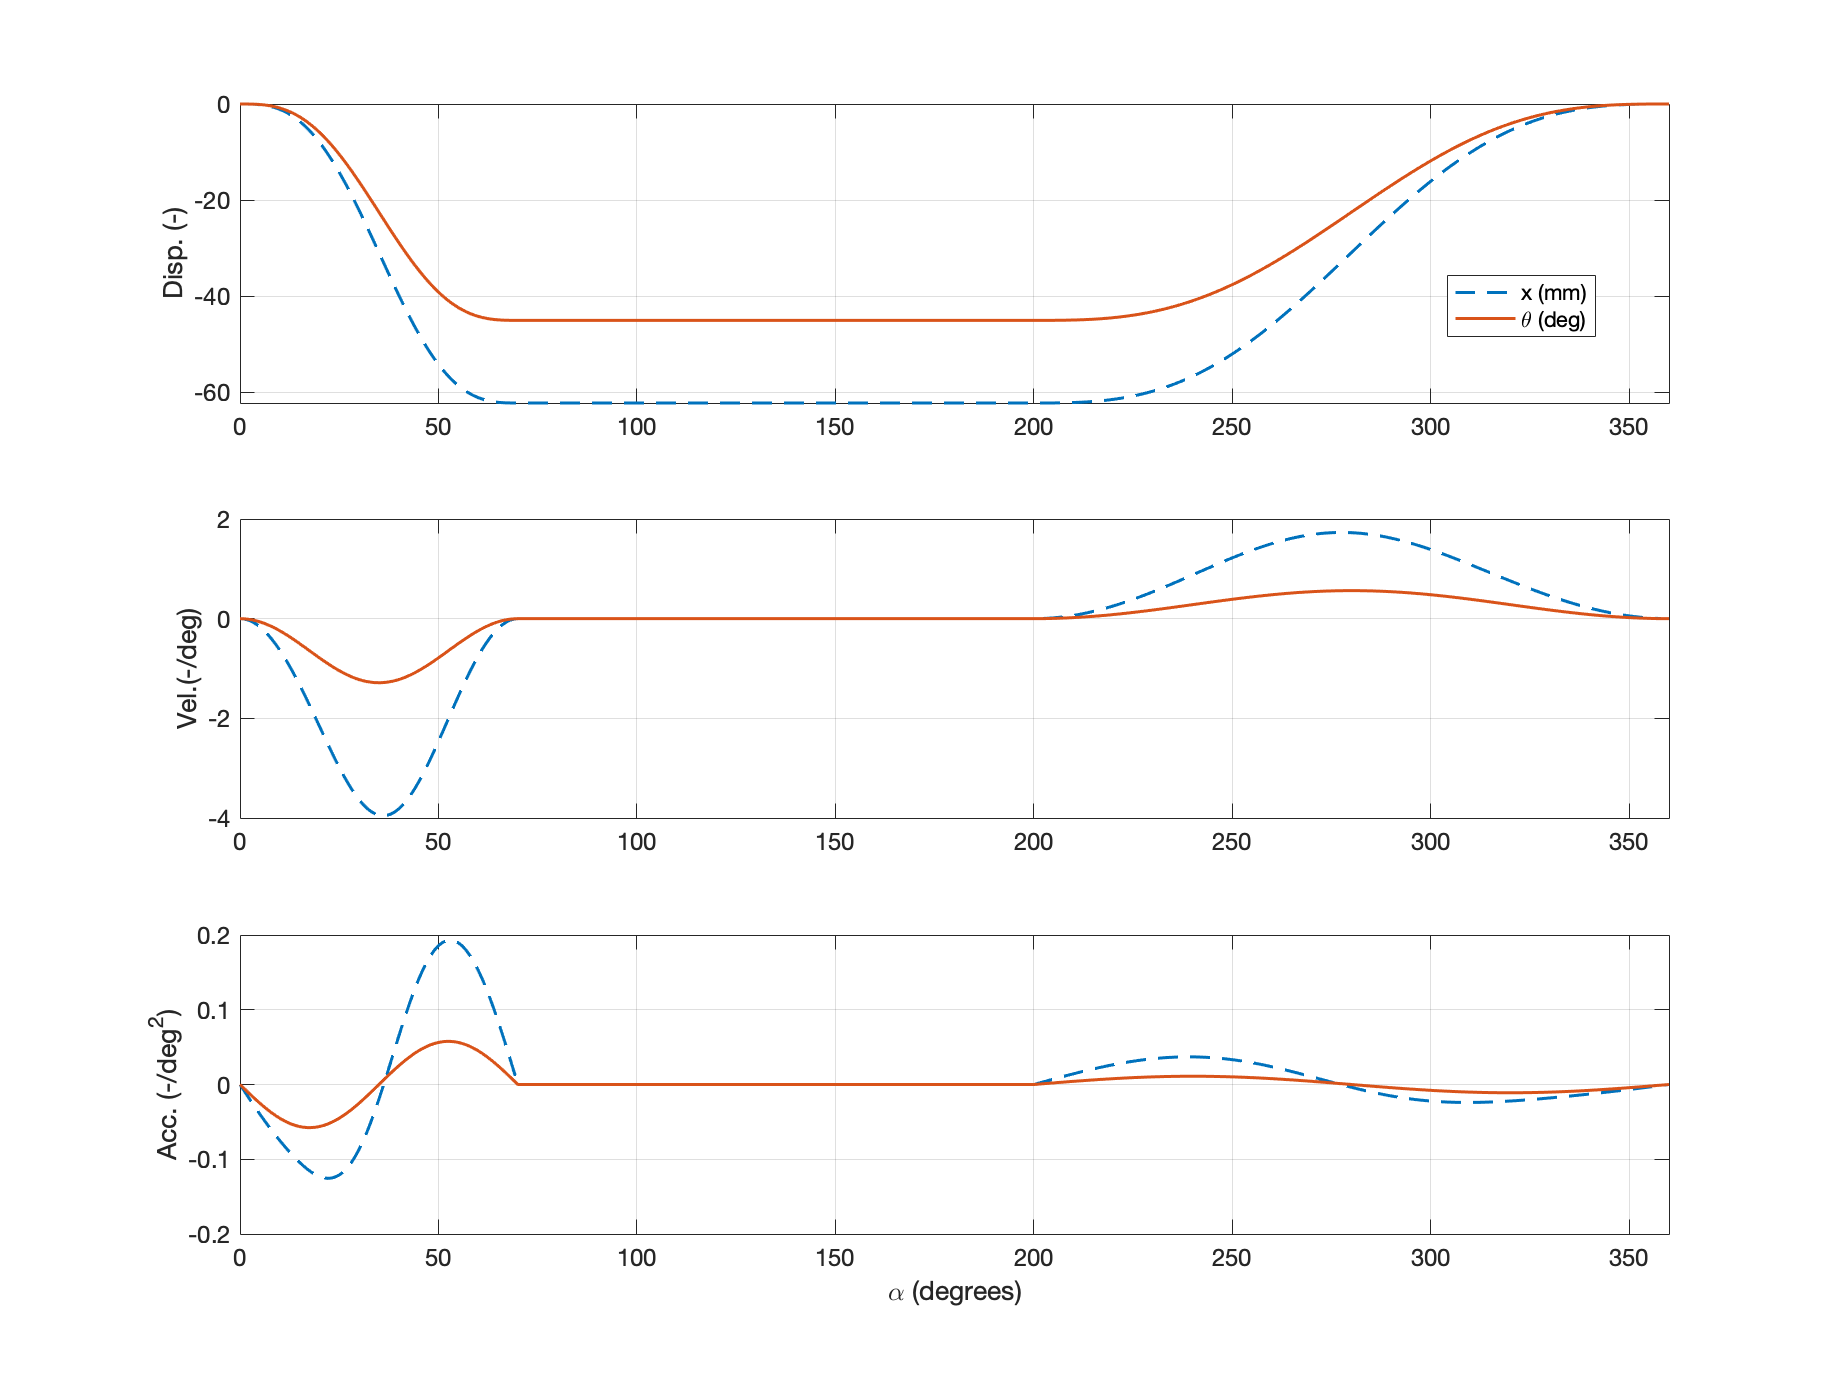
\includegraphics[width=1\textwidth]{Pictures/motionLaw.png}
	\caption{Motion law for both $x$ (in blue) and $\theta$ (in red) with cycloidal choices.}
	\label{fig: cic motion laws}
\end{figure}

With the above motion law, we checked for the transmission angle, given by Fig.~\ref{fig: trans angle}; it varies from 76 til 84 degrees (a good transmission angle is above 45$^\circ$).
\begin{figure}
	\centering
	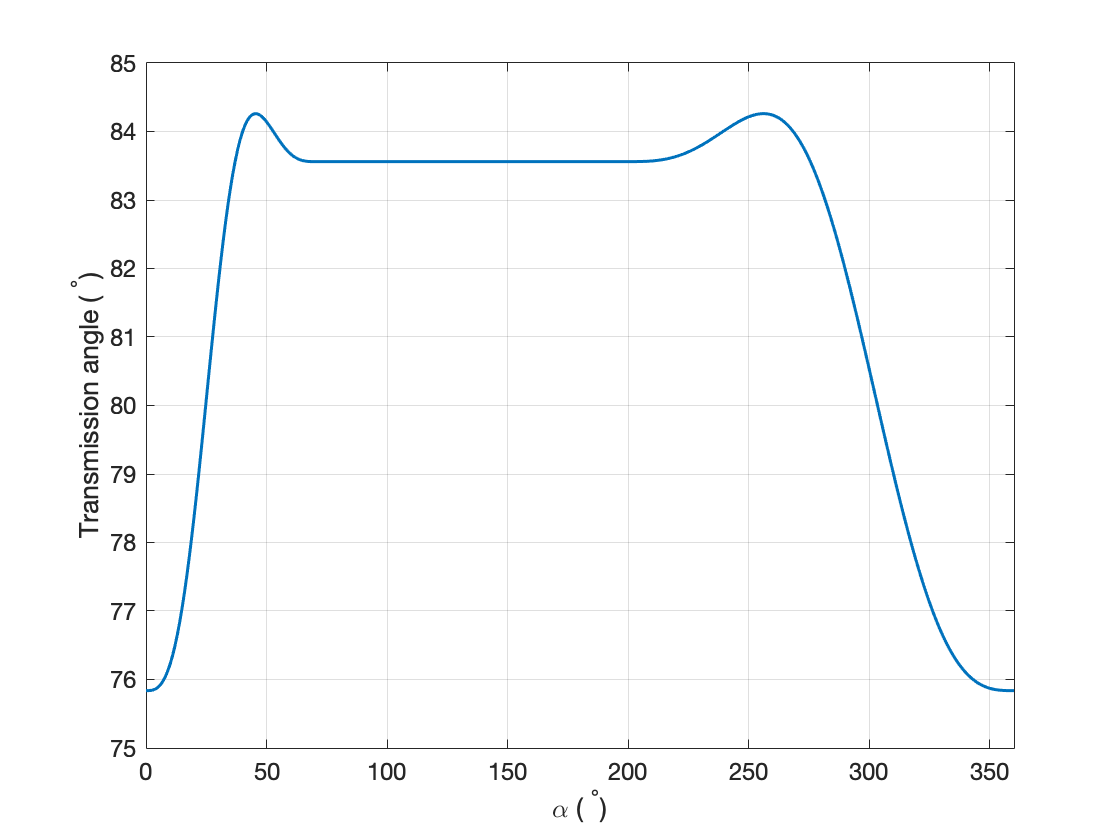
\includegraphics[width=0.8\textwidth]{Pictures/transmissionAngle.png}
	\caption{Transmission angle of the slider-crank mechanism.}
	\label{fig: trans angle}
\end{figure}
 
 Thus, we design the translational cam with the equations in \eqref{exp: cam profile}. We remember that $x$ is positive to the right and that the contact point of our cam is at the left, thus a negative sign in the x-coordinate of the cam has to be added in order to obtain the right cam. Furthermore, the cam should then rotate counter-clockwise. The respective motion law is depicted at Fig.~\ref{fig: transl cam}. 
\begin{figure}[htbp!]
	\centering
	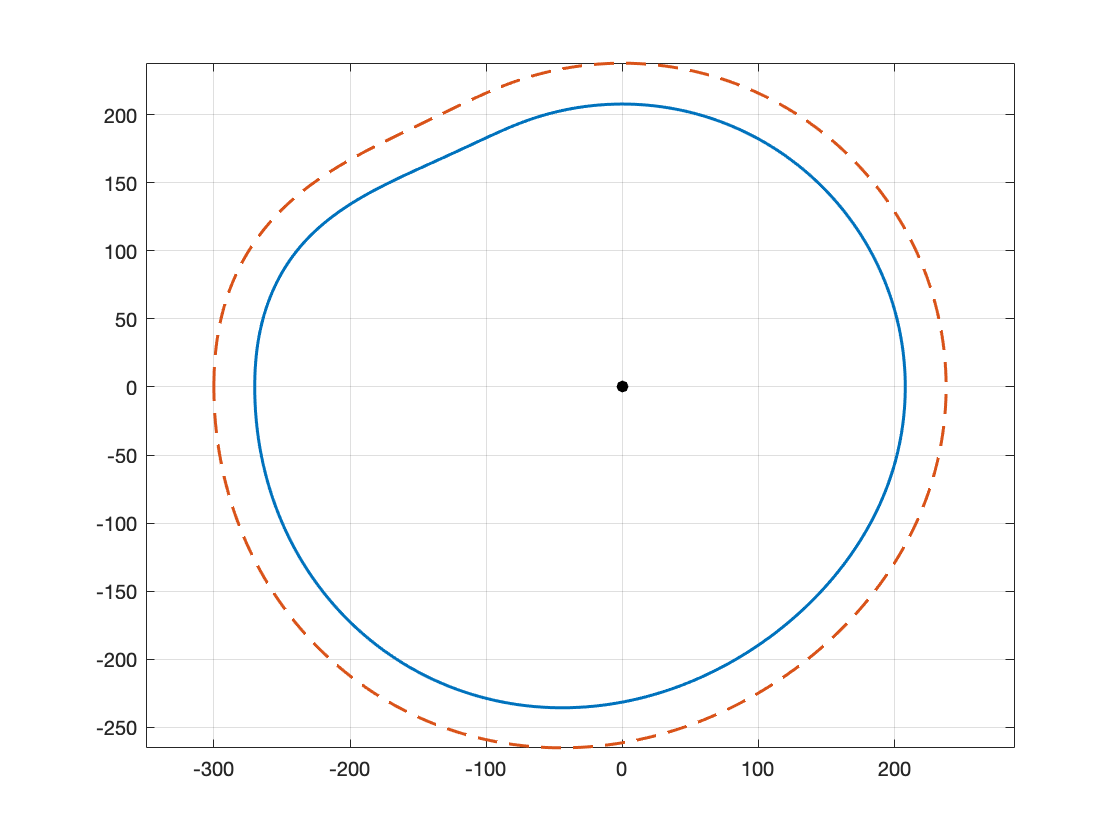
\includegraphics[width = 0.8\textwidth]{Pictures/transCam}
	\caption{Translational cam generated for the first motion law (cycloidal motions).}
	\label{fig: transl cam}
\end{figure}
For this corresponding stroke, we choose a base radius $R_{b0} = \SI{300}{\milli\metre}$ and a roller radius $R_r = \SI{30}{\milli\metre}$, that seemed reasonable to keep the pressure angle under control (for the given motion law) and to avoid undercut. Fig.~\ref{fig: pressure angle} shows how the pressure angle between the cam and the follower varies as function of the master angle. It is kept bound and its maximum value is less than $45$ degrees. Fig.~\ref{fig: curvature}.a shows the curvature of the both the pitch and cam profile, while the Fig.~\ref{fig: curvature}.b plots $\rho \cdot \rho_0$ vs $\alpha$. If $\rho\cdot\rho_0 < 0$ the undercut occurs. From the plot, it's clear (any trespassing of the middle axis would have been graphically accused) that no undercut takes place here.
\begin{figure}[htbp!]
	\centering
	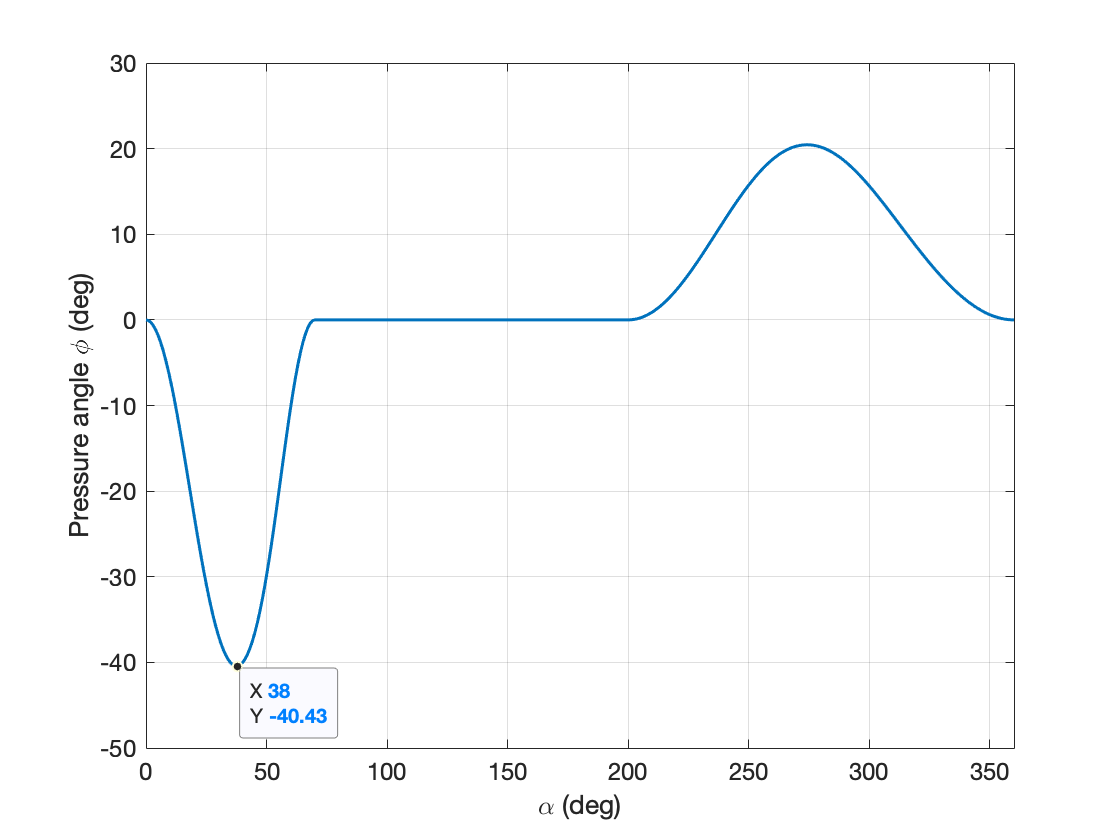
\includegraphics[width=0.6\textwidth]{Pictures/pressAngle}
	\caption{Pressure angle related to the first cam-follower system.}
	\label{fig: pressure angle}
\end{figure}
\begin{figure}[htbp!]
	\centering
	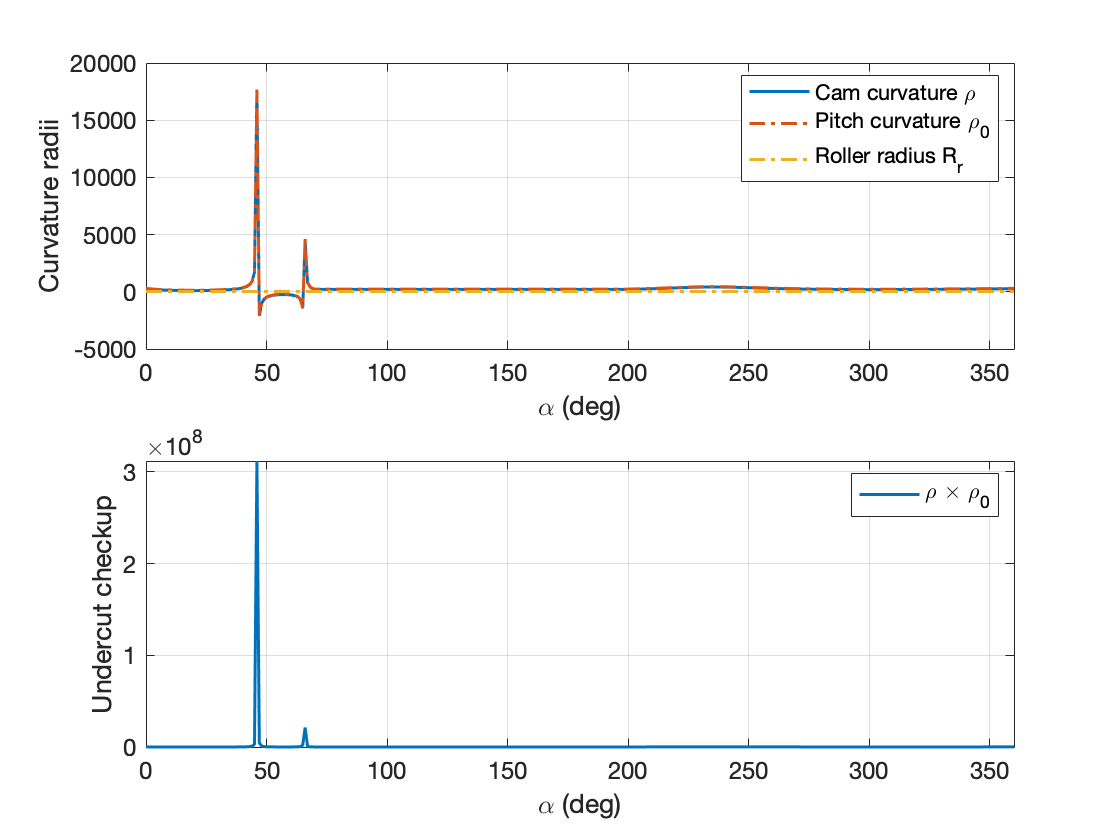
\includegraphics[width=0.8\textwidth]{Pictures/undercutCondition}
	\caption{Curvature radius and undercut condition check.}
	\label{fig: curvature}
\end{figure}


\FloatBarrier
\section{Discussion}

\end{document}